A wildlife ecologist measured $x_{1} =$ tail length (in millimeters) and $x_{2} =$ wing length (in millimeters) for a sample of $n = 45$ female hook-billed kites.
These data are displayed in Table 5.12.
Using the data in the table,

\begin{enumerate}[label= (\alph*)]
    \item Find and sketch the 95\% confidence ellipse for the population means $\mu_{1}$ and $\mu_{2}$.
    Suppose it is known that $\mu_{1} = 190 \text{mm}$ and $\mu_{2} = 275 \text{mm}$ for male hook-billed kites. 
    Are these plausible values for the mean tail length and mean wing length for
    the female birds?
    Explain.

    \begin{figure}[H]
        \centering
        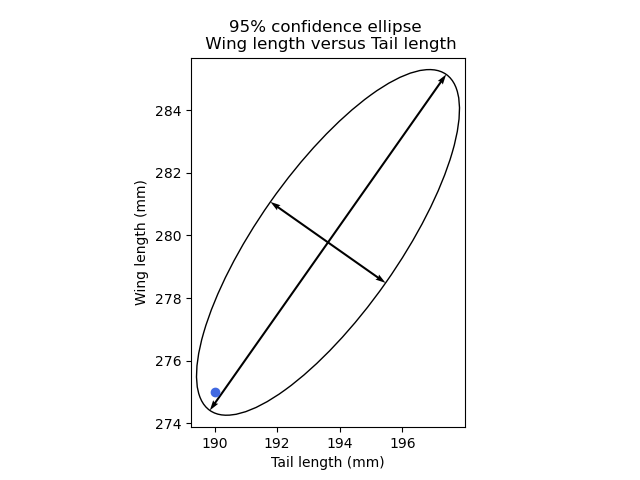
\includegraphics[scale=0.65]{./python/chapter-5/Question-5-20-a.png}
    \end{figure}

    The values exist within the confindence ellipse for male birds, and so, are plausable values for male birds.
    We don't have any data on female birds, so there's no way to say anything about the plausibility of the values in relation to females.

    \item Construct the simultaneous 95\% $T^{2}$-intervals for $\mu_{1}$ and $\mu_{2}$ and the 95\% Bonferroni
    intervals for $\mu_{1}$ and $\mu_{2}$. Compare the two sets of intervals. What advantage, if any, do
    the $T^{2}$-intervals have over the Bonferroni intervals?
    \[
        \bar{\textbf{x}}
        =
        \begin{bNiceArray}{c}
            193.62 \\
            279.78
        \end{bNiceArray}
        \hspace{0.20cm}
        \text{and}
        \hspace{0.20cm}
        \textbf{S}
        =
        \begin{bNiceArray}{cc}
            120.69 & 122.35 \\
            122.35 & 208.54
        \end{bNiceArray}
    \]
    The 95\% $T^{2}$ simultaneous confidence intervals:
    \[
    \bar{x}_{i}
    \pm
    \sqrt{
        \frac{(n-1)p}{(n-p)}
        F_{p, n-p}\left(\alpha\right)
    }
    \sqrt{
        \frac{s_{ii}}{n}
    }
    \]

    \[
        \begin{NiceArray}{rrrr}
           193.62 \pm \sqrt{6.58} \frac{\sqrt{120.69}}{\sqrt{45}} & \text{contains } \mu_{1} & \text{ or } & 189.42 \leq \mu_{1} \leq 197.82 \\
           279.78 \pm \sqrt{6.58} \frac{\sqrt{208.54}}{\sqrt{45}} & \text{contains } \mu_{2} & \text{ or } & 274.26 \leq \mu_{2} \leq 285.30 \\
        \end{NiceArray}
        \]

    The 95\% Bonferroni confidence intervals:
    \[
        \bar{x}_{i}
        \pm
        t_{n-1}
        \left(\frac{\alpha}{2m}\right)
        \sqrt{
            \frac{
                    s_{ii}
                }{
                    n
                }
            }
    \]

    \[
        \begin{NiceArray}{rrrr}
           193.62 \pm 2.32 \frac{\sqrt{120.69}}{\sqrt{45}} & \text{contains } \mu_{1} & \text{ or } & 189.82 \leq \mu_{1} \leq 197.42 \\
           279.78 \pm 2.32 \frac{\sqrt{208.54}}{\sqrt{45}} & \text{contains } \mu_{2} & \text{ or } & 274.78 \leq \mu_{2} \leq 284.77 \\
        \end{NiceArray}
    \]

    As we already known, the Bonferroni interval is more narrow than the simultaneous $T^{2}$. This time only slightly though. The $T^{2}$ intervals are preferred to the Bonferroni intervals when we wish to incorporate the correlation between tail length and wing length into the interval.

    \item Is the bivariate normal distribution a viable population model? Explain with reference to \textit{Q-Q} plots and a scatter diagram.
    
    \begin{figure}[H]
        \centering
        \begin{tabular}{cc}
            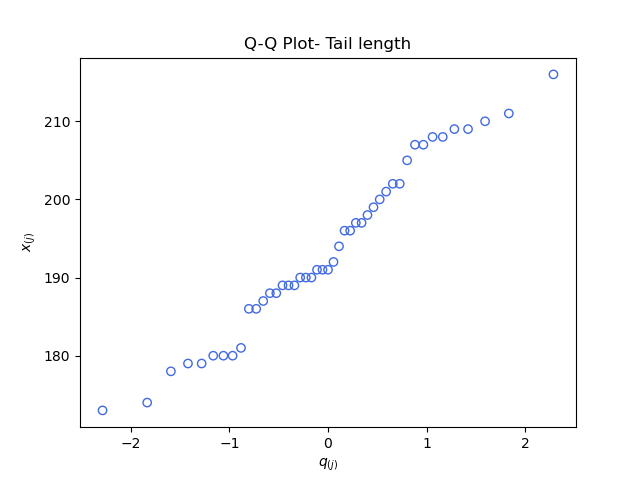
\includegraphics[scale=0.30]{./python/chapter-5/Question-5-20-c-QQ-TailLen.png} &
            \includegraphics[scale=0.30]{./python/chapter-5/Question-5-20-c-QQ-Winglen.png}
        \end{tabular}
    \end{figure}

    \begin{figure}[H]
        \centering
        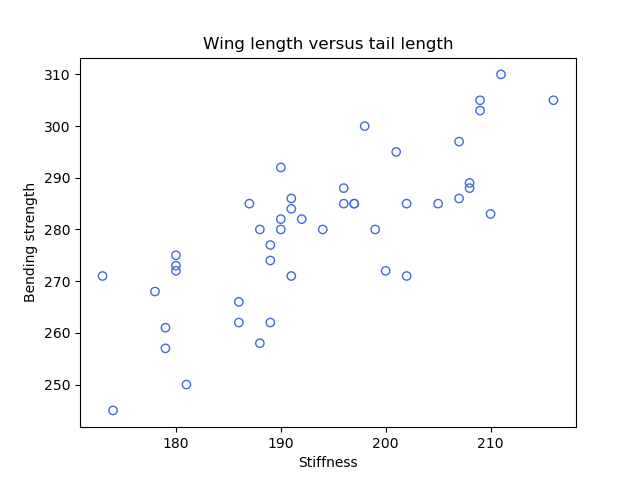
\includegraphics[scale=0.55]{./python/chapter-5/Question-5-20-c-xy.png}
    \end{figure}

    The \textit{Q-Q} plots look fairly linear, so the data is normally distributed in univariate cases. The scatterplot of wing length versus tail length shows a positive trend with a roughly elliptical shape. The elliptical shape isn't perfect, there may be some outliers. Because of these things we could consider tail length and wing length to be bivariate normal. 

\end{enumerate}